\chapter{Applying Blockchain}
\lable{blockchain}
\section{Implementation}
As can be seen in Figure 1, each "block" consists of three values: the hash of the previous block, the data we want to have a verifiable record of, and a Nonce, or random number. Blocks are then hashed--- depending on the need for hashing difficulty (Proof-of-Work) they will have a certain number of 0 bits at the beginning of the hash. In order to create a different hash (If a hash of the required format is not initially found) the nonce is changed via incrementing or a random number generator. The time a block hash was found is recorded, and the hash and time are published, using one of three methods described in section 2. Traditionally, Bitcoin makes the amount of work needed to find a hash for a block average about 10 minutes \cite{Bitcoin}, but the need for Proof-of-Work depends on the method of publication and verification.
        
        \begin{figure}[hbt!]
        \centering
        \makebox[\textwidth][c]{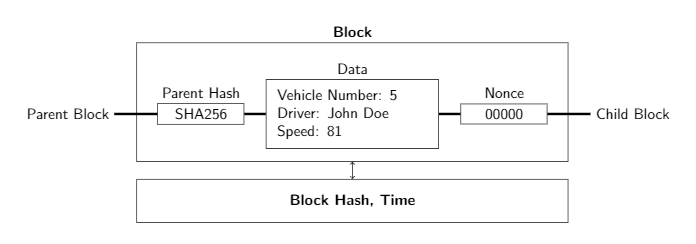
\includegraphics[width=1.1\textwidth]{blocc.png}}%
        \caption{Anatomy of a Block}
        \end{figure} %block anatomy

        Users in need of log verification can then hash the block themselves to verify that the public record of the block matches the hash they generated. If it does not, they know that the data in that block, or a block before it, has been tampered with. If the hash does not line up, the user can hash each block starting from the most recent and working their way back. The start of the data that has been tampered with will be in the first block in the chain that does not validate with the public record. This means that you can still trust the integrity of the logs that occurred before the corrupted block, hence there is not a total data loss, unlike legacy systems without blockchain log authentication.
        
        The blockchain will sit between the software that grabs the data from the GeoTab Server and the Neutral Vehicle server, and send its results to the Neutral Vehicle server and the Neutral Vehicle database. This information should be available to users who query data from the Neutral Vehicle Server.

\begin{figure}[hbt!]
\centering
  \makebox[\textwidth][c]{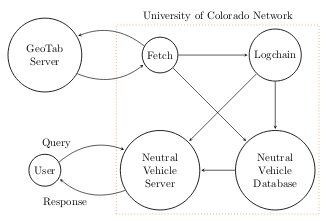
\includegraphics[width=0.5\textwidth]{network.png}}%
  \caption{Neutral Vehicle Network}
\end{figure}

\subsection{Anchor Blocks}
        \begin{figure}[hbt!]
        \centering
        \makebox[\textwidth][c]{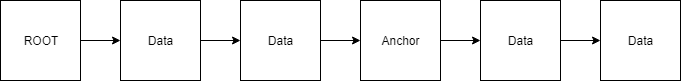
\includegraphics[width=1\textwidth]{chain.png}}%
        \caption{Anchor Blocks on a Chain}
        \end{figure} %block chain
        
        It is ultimately infeasible to keep all log data from all systems forever. This means that old logs on systems need to be periodically deleted, but this would cause all the blocks to be declared invalid. In our software, we suggest a solution to the need for log deletion with Anchor blocks.   Anchor blocks are placed in the middle of the blockchain (Fig. 2), and are identical in function to a ROOT block, and do not need to be authenticated as they carry no data. Any blocks before an Anchor block do not effect the validity of the Anchor block, and any blocks after it build off of the Anchor block's default valid status. This means that as log data is periodically deleted for system space, we can remove sections of the blockchain up to Anchor blocks without needing to worry about the rest of the log being declared invalid.
        
        Another benefit of Anchor blocks is that authentication can be performed much faster because an authentication scan for any given block B needs to only go back to the nearest Anchor block to prove validity. Normally, all blocks back to ROOT would need to be verified to authenticate B, which is a costly and time-consuming computation. Anchor blocks make that computation a fraction of the time and resources.
        
        
        
         \section{Blockchain Authenticity Verification}
In this section I propose three methods for publishing the data to verify and validate blocks for third parties. Each has their pros and cons. 
\subsection{Storage on Etherium}{
The size of a file that consists of a SHA256 hash, nonce, and date is roughly 12 Words. The price to store a single Kilobyte on the Etherium Blockchain is 24,000 Gas \cite{EthCosts}. The Gas-to-Ether conversion ratio is 1 Gas = 2.4 Gwei = 0.0000000024 ETH. Therefore, the amount of Ether needed to store 12 Words of data on Etherium is 0.00048. 1 ETH = \$123 USD. That means, to store 4 Kilobytes of information on the Etherium Blockchain is \$0.0283392 USD \footnote{All prices are current as of 2/15/2019}. Depending on how often blocks are finalized, hashed, and added to the chain, this could cost between \$0.02, if you only create one block a day, to \$345.60 a day, if you create a block every 5 seconds. 
\begin{figure}[hbt!]
    \centering
\begin{tikzpicture}
\begin{axis}[
    axis lines = left,
    xlabel = {Blocks/Minute},
    ylabel = {$Cost (\$)$},
]
\addplot [
    domain=0:60, 
    samples=100, 
    color=red,
]
{0.0283392*x};
\end{axis}
\end{tikzpicture}
    \caption{The Blocks-To-Cost Ratio}
    \label{fig:my_label}
\end{figure}

The trade off between creating blocks quickly vs. slowly is the security of the data. If only one block is created a day, that gives attackers an entire day to modify the data. However, if a block is created every 5 seconds, there is very little time for an attacker to modify the data.

\textbf{Pros:} The data is very public, and uneditable once published.

\textbf{Cons:} Costs money, and the primary trade-off is between cost and security.
}
\subsection{Node Distribution}{Another possibility is making users who want to use the software for log validation run a node of the blockchain--- this would mimic the format of Bitcoin, because of the distributed nature of the log, each node would keep a copy of the chain and other users would use the collective agreement on the blockchain to verify the authenticity of logs. \cite{Bitcoin}
Unfortunately this option may not work for Neutral Vehicle because of the centralized server, at least in the early stages.

\textbf{Pros:} No money needed, relatively secure without a need for additional measures.

\textbf{Cons:} Need for additional users willing to contribute to the blockchain.
}

\subsection{Central Authority}{The cheapest, and easiest way to authenticate the blockchain is to have a central authority, in this case, the Neutral Vehicle servers. Having the validating data from blocks sent to (or created on) this server, which are then signed by a Neutral Vehicle private key and posted to an online database of block hashes for anyone to view is the cheapest method of creating verification for third parties. However, this does come with security issues--- if the server is attacked and security breached, attackers will have the ability to steal the Neutral Vehicle private key and re-hash any data they want, and replace the old data with the new data on the public database. The impact of such a breach can be reduced by having a secondary server that validates all posted hashes with its own private copy.

\textbf{Pros:} Cheap, easy, and effective.

\textbf{Cons:}Much more vulnerable to malicious attacks on the centralized server. The use of a central authority goes against the initial reason for the creation of blockchain.
}

In this thesis we used a central authority as the verification method. 
        
\subsection{Blockchain Security}

    The fundamental security of blockchain lies in the resource-intensive hashing process. Of course, the security provided by the resource-intensive hashing process is dependent on the difficulty of hashing, how often blocks are created, and the amount of compute power available to both the attacker and the blockchain. Ideally the blockchain would also be distributed via the Node Distribution verification method addressed in section 4.3.2, but 
    
    \begin{figure}[hbt!]
    \centering

    \makebox[\textwidth][c]{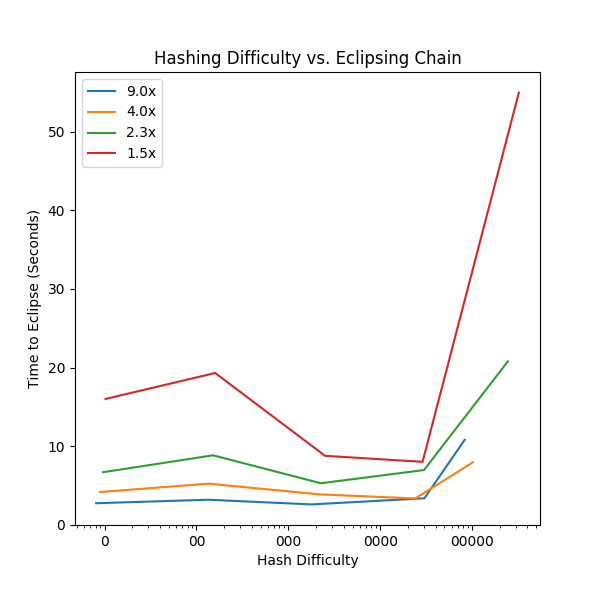
\includegraphics[width=1\textwidth]{hashDiff.png}}%

    \caption{The CPU power needed for an attacker to overwhelm the blockchain }
    \label{fig:security}
\end{figure}

 \begin{figure}[hbt!]
    \centering
    \makebox[\textwidth][c]{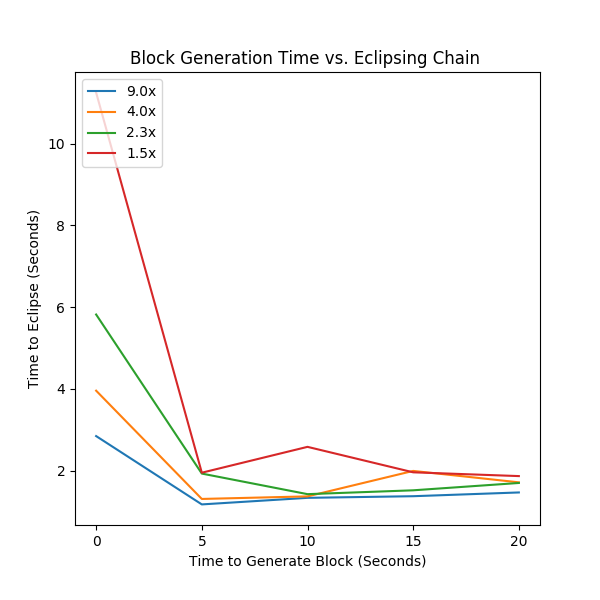
\includegraphics[width=1\textwidth]{blockTime.png}}%

    \caption{The CPU power needed to hash the blockchain as the server}
    \label{fig:passiveReqs}
\end{figure}
    
    
    
    \subsubsection{Anchor Block Security}
    When proposing anchor blocks, we realized we don't actually know how secure they are. In fact, they may pose a significant risk towards the health of the chain and attackers' abilities to modify or delete data. 
        
        
        
        
        \section{Limitations and Interdisciplinary Approach}     
         The software we propose is meant to protect against log deletion and log modification. This does not include protecting against attackers modifying the hardware to report false data, or protection of the data in transmission from the hardware to the server. Unfortunately, log verification with blockchain only tells users where the log was modified or deleted, but not how it was changed. Instead, this is inferred using interdependencies within the data. By using correlations in vehicular data between metrics such as distance traveled, miles-per-gallon, or GPS location, then we can identify what data has been modified because the log does not have internal consistency.
         
         
         
         
         
         